
Imagine a system of $N$-particles, $\alpha = 1, ... , N$, with masses $m_\alpha$ and positions $\vec{r}_\alpha$ relative to an arbitrary origin $O$. The {\bfseries center of mass} ({\bfseries CM}) is defined as the position relative to the origin $O$,

\begin{equation*}
    \vec{R} = \frac{1}{M} \sum^{N}_{\alpha = 1} m_\alpha \vec{r}_\alpha = \frac{m_1 \vec{r}_1 + ... + m_\alpha \vec{r}_\alpha}{M}
\end{equation*}

\noindent where $M$ is the total mass of the particles. Note that CM is a vector equation; therefore, it can be broken into its components. For example, in the x-direction:

\begin{equation*}
    CM_x = \frac{1}{M} \sum^{N}_{\alpha = 1} m_\alpha x_\alpha.
\end{equation*}

We also note the relationship between the mass and position of each particle. The CM is weighted (by $m_\alpha$) of the particles position. An example of this is the Sun-Earth system shown in figure \ref{fig:cm-sun-earth}. In a 2-body system such as this, the center of mass is,

\begin{equation*}
    \vec{R} = \frac{m_{sun} \vec{r_{sun}} + m_{earth} \vec{r}_{earth}}{m_{sun} + m_{earth}}
\end{equation*}

We know that $m_{sun} \gg m_{earth}$ meaning $\vec{r}$, the center of mass vector, will be closer to $m_{sun}$. In fact the mass of the Sun is so much greater than the mass of the Earth, it is a good approximation to place the CM where the Sun is located.

\begin{figure}[h]
    \centering
    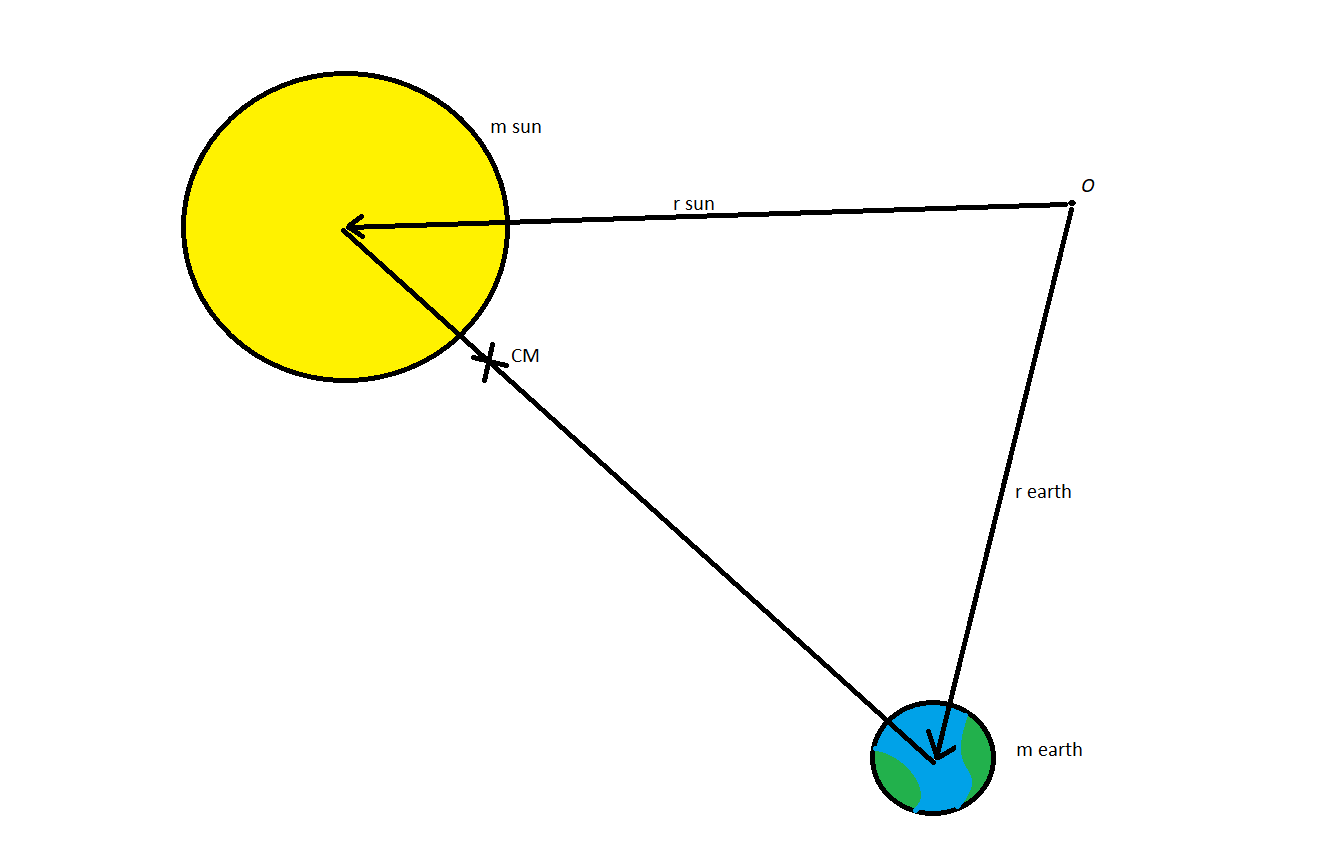
\includegraphics[width=6cm]{Classical_Mechanics/2.5-center-of-mass/cm-sun-earth.png}
    \caption{The center of mass of the Sun-Earth system.}
    \label{fig:cm-sun-earth}
\end{figure}

Writing the total momentum $\vec{P}$ of any $N$-particle system,

\begin{equation*}
    \vec{P} = \sum^{N}_{\alpha = 1} m_\alpha \dot{\vec{r}}_\alpha = M \dot{\vec{R}}.
\end{equation*}

This equation means the total momentum of $N$-particles is equal to the product of a single particle with mass $M$ and velocity of the CM $\dot{\vec{R}}$. Therefore, you can treat a large amount of particles as a single particle traveling at the center of mass.

Similarly, $\dot{\vec{P}} = M \ddot{\vec{R}} = \vec{F}_{ext}$. This states that the center of mass of the particles moves exactly as if it was a single particle mass being subjected to the net external force of the system. Hence, we treat large, irregular bodies, such as baseballs and planets as if they are point masses. This is a decent approximation if the trajectory is much larger than the size of the object.

You can follow the equation above to calculate CM or, if the mass is continuously distributed over a body,

\begin{equation*}
    \vec{R} = \frac{1}{M} \int \vec{r} dm = \frac{1}{M} \int \delta \vec{r} dV
\end{equation*}

\noindent where $dm$ is an element of mass, $\delta$ is the mass density of the body, and $dV$ is an element of volume. An example of this is shown below.

% ------- EXAMPLE: CENTER OF MASS SOLID CONE
{\exbegin Example 2.5: Center of Mass of a Solid Cone}

\begin{figure}[h]
    \centering
    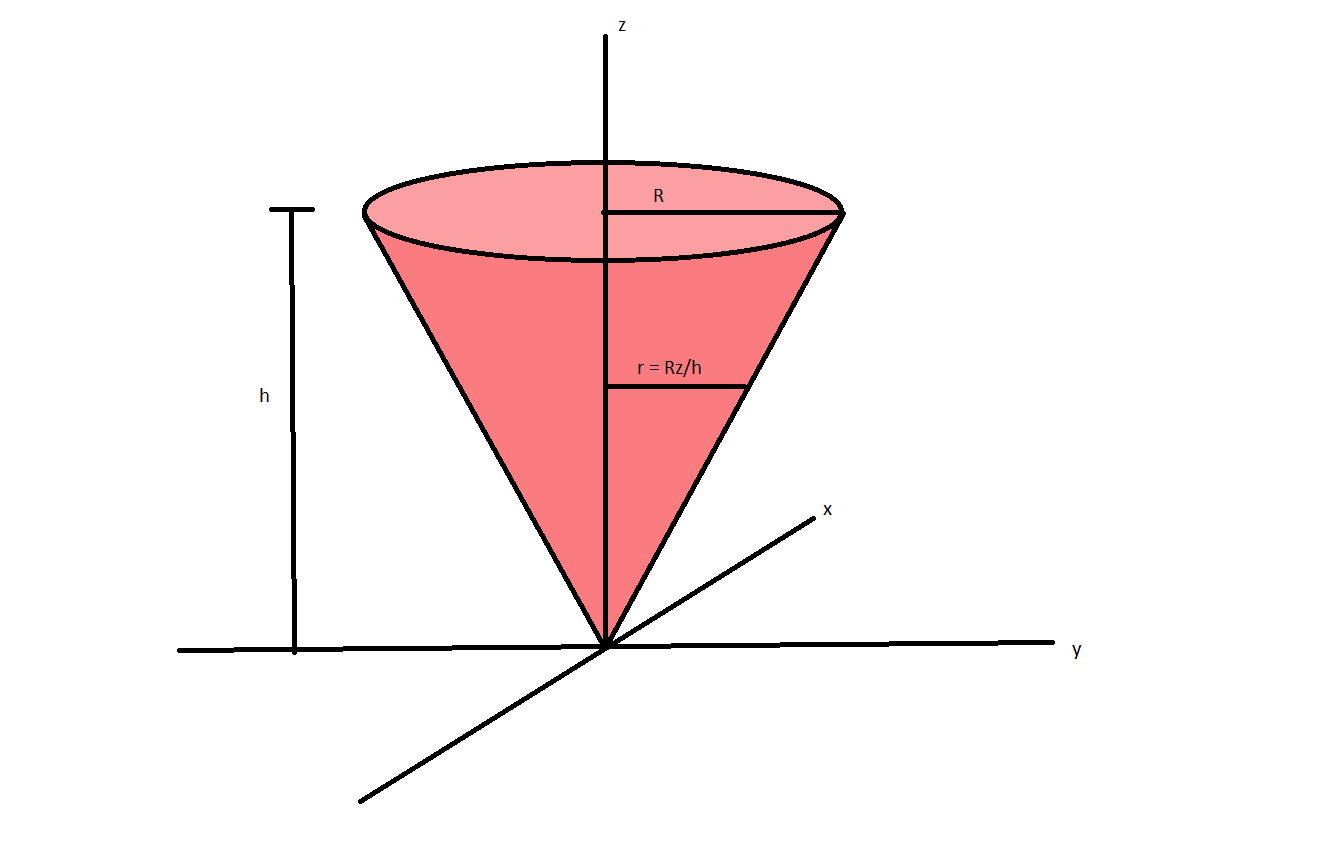
\includegraphics[width=13cm]{Classical_Mechanics/2.5-center-of-mass/ex-cm-cone.png}
    \caption{Cone for Example 2.5.}
    \label{fig:ex-cm-cone}
\end{figure}

Find the CM position of a uniform solid cone (shown in figure \ref{fig:ex-cm-cone}) that is symmetrical on the z-axis. By intuition, the CM will be along the z-axis, that is $CM_x = CM_y = 0$. To find the CM along the z-axis, we need to solve the integral,

\begin{equation*}
    CM_z = \frac{1}{M} \int \delta z dV = \frac{\delta}{M} \int z dx dy dz.
\end{equation*}

\noindent where $\delta$ is constant and $dV = dx dy dz$. For a given z, the integral over x and y runs over a circle of radius $Rz/h$,

\begin{equation*}
    CM_z = \frac{\delta}{M} \int dxdy \int z dz \rightarrow \frac{\delta}{M} \pi (Rz/h)^2 \int^h_0 zdz.
\end{equation*}

In the above equation, $\int dx dy = \pi r^2$, where $r = Rz/h$, or the area of a horizontal slice in the cone. Solving this last equation yields,

\begin{equation*}
    \frac{\delta}{M} \pi (Rz/h)^2 \int^h_0 zdz \rightarrow \frac{\delta \pi R^2}{M h^2} \int^h_0 z^3 dz = \frac{\delta \pi R^2 h^4}{4 M h^2} = \frac{\delta \pi R^2 h^2}{4 M}.
\end{equation*}

Finally, replacing $M = \delta \times V = \frac{1}{3} \delta \pi R^2 h$,

\begin{equation*}
    CM_z = \frac{\delta \pi R^2 h^2}{4 M} = \frac{3}{4}h
\end{equation*}

{\exend}
